\subsection{Sequence Diagram}

\begin{figure}[H]
    \centering
    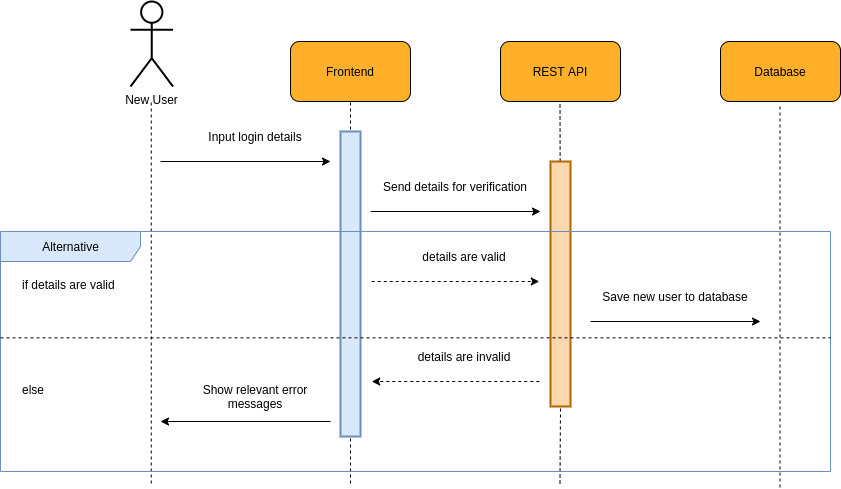
\includegraphics[scale=0.5]{./diagrams/sequence/seq-01.png}
    \caption{Sequence Diagram of UC-1}
    \label{fig:seq-01}
    
\end{figure}


\begin{figure}[H]
    \centering
    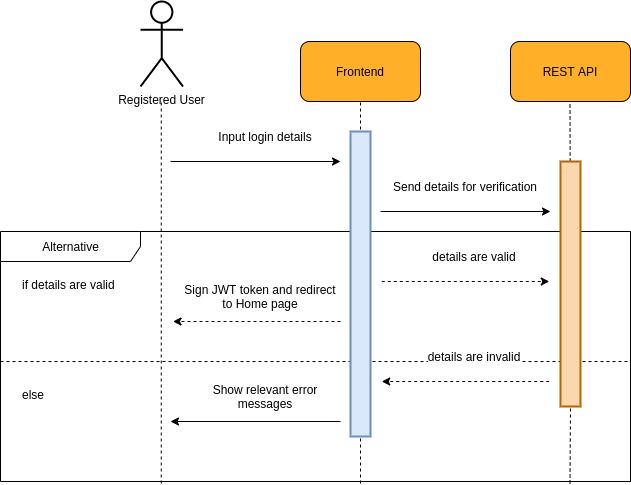
\includegraphics[scale=0.5]{./diagrams/sequence/seq-02.png}
    \caption{Sequence Diagram of UC-2}
    \label{fig:seq-02}
    
\end{figure}


\begin{figure}[H]
    \centering
    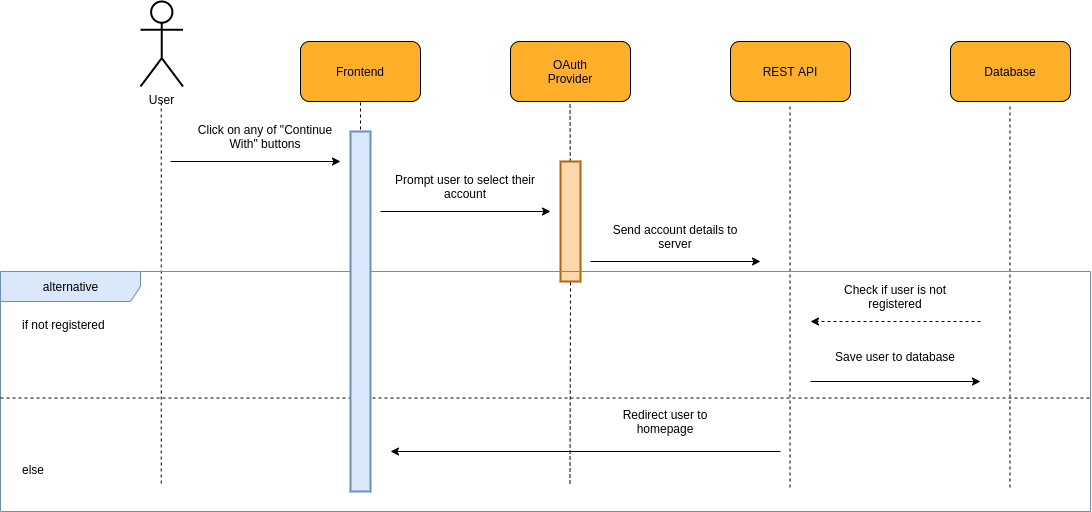
\includegraphics[scale=0.5]{./diagrams/sequence/seq-03.png}
    \caption{Sequence Diagram of UC-3}
    \label{fig:seq-03}
    
\end{figure}


\begin{figure}[H]
    \centering
    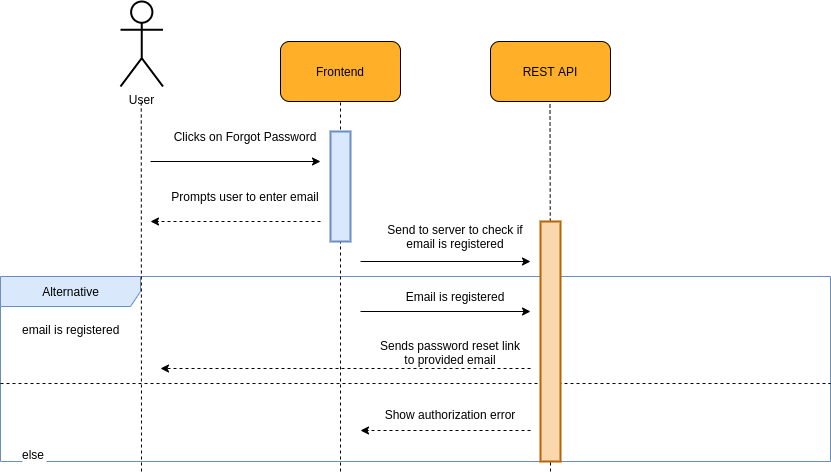
\includegraphics[scale=0.5]{./diagrams/sequence/seq-04.png}
    \caption{Sequence Diagram of UC-4}
    \label{fig:seq-04}
    
\end{figure}


\begin{figure}[H]
    \centering
    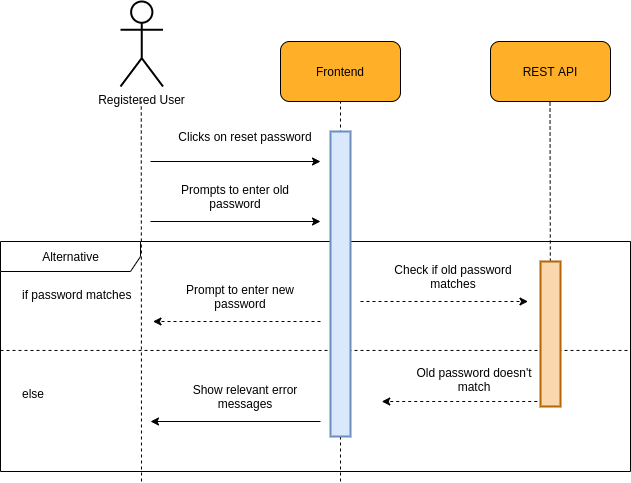
\includegraphics[scale=0.5]{./diagrams/sequence/seq-05.png}
    \caption{Sequence Diagram of UC-5}
    \label{fig:seq-05}
    
\end{figure}


\begin{figure}[H]
    \centering
    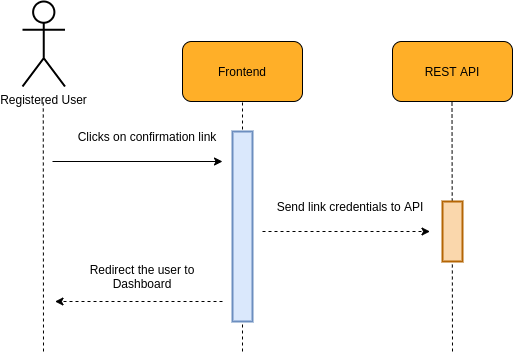
\includegraphics[scale=0.5]{./diagrams/sequence/seq-06.png}
    \caption{Sequence Diagram of UC-6}
    \label{fig:seq-06}
    
\end{figure}


\begin{figure}[H]
    \centering
    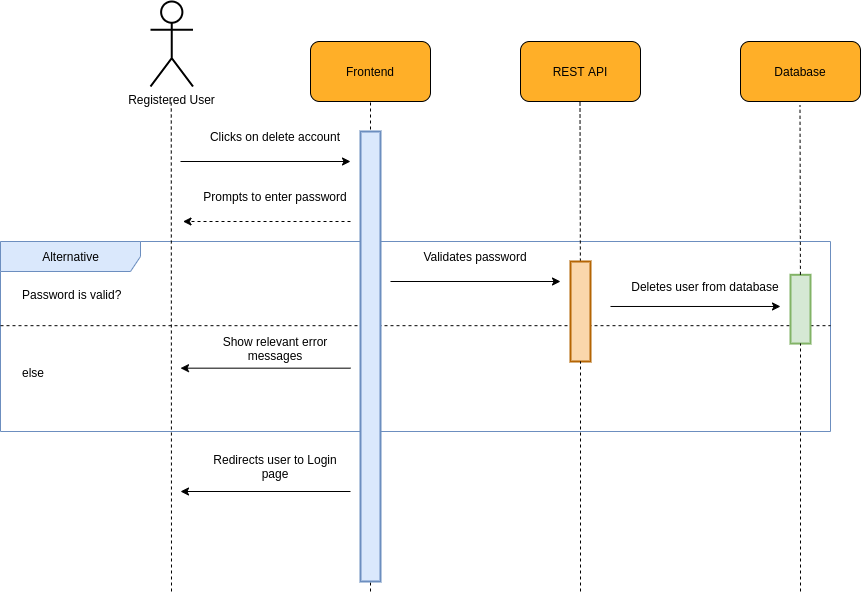
\includegraphics[scale=0.5]{./diagrams/sequence/seq-07.png}
    \caption{Sequence Diagram of UC-7}
    \label{fig:seq-07}
    
\end{figure}


\begin{figure}[H]
    \centering
    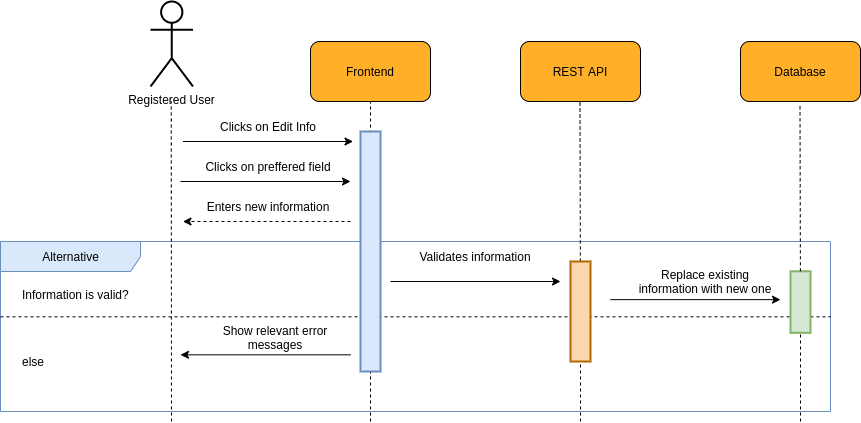
\includegraphics[scale=0.5]{./diagrams/sequence/seq-08.png}
    \caption{Sequence Diagram of UC-8}
    \label{fig:seq-08}
    
\end{figure}


\begin{figure}[H]
    \centering
    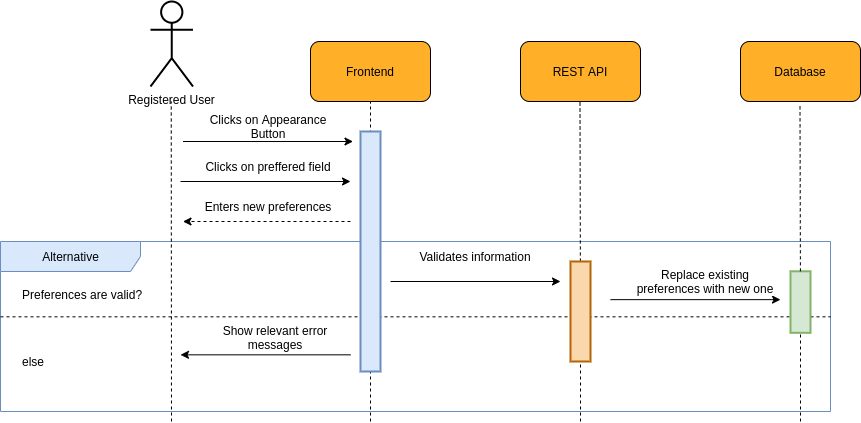
\includegraphics[scale=0.5]{./diagrams/sequence/seq-09.png}
    \caption{Sequence Diagram of UC-9}
    \label{fig:seq-09}
    
\end{figure}


\begin{figure}[H]
    \centering
    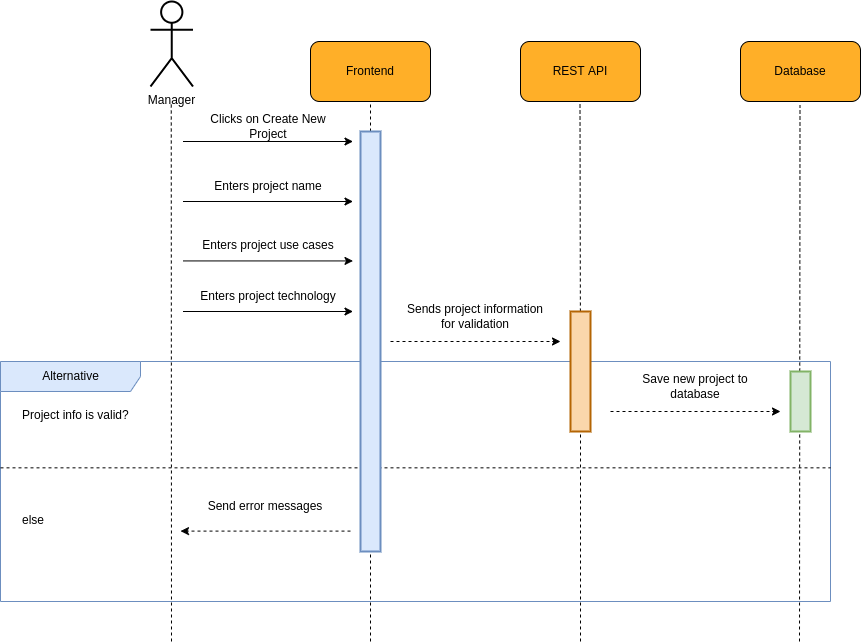
\includegraphics[scale=0.5]{./diagrams/sequence/seq-10.png}
    \caption{Sequence Diagram of UC-10}
    \label{fig:seq-10}
    
\end{figure}


\begin{figure}[H]
    \centering
    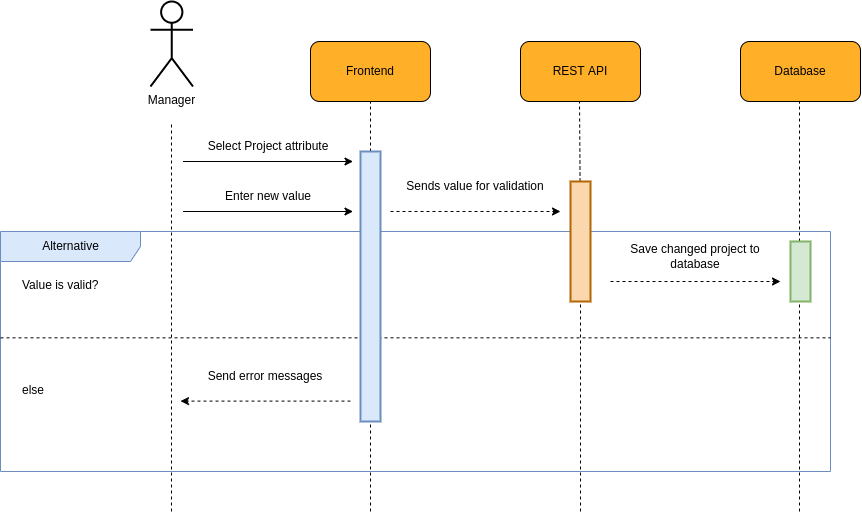
\includegraphics[scale=0.5]{./diagrams/sequence/seq-11.png}
    \caption{Sequence Diagram of UC-11}
    \label{fig:seq-11}
    
\end{figure}


\begin{figure}[H]
    \centering
    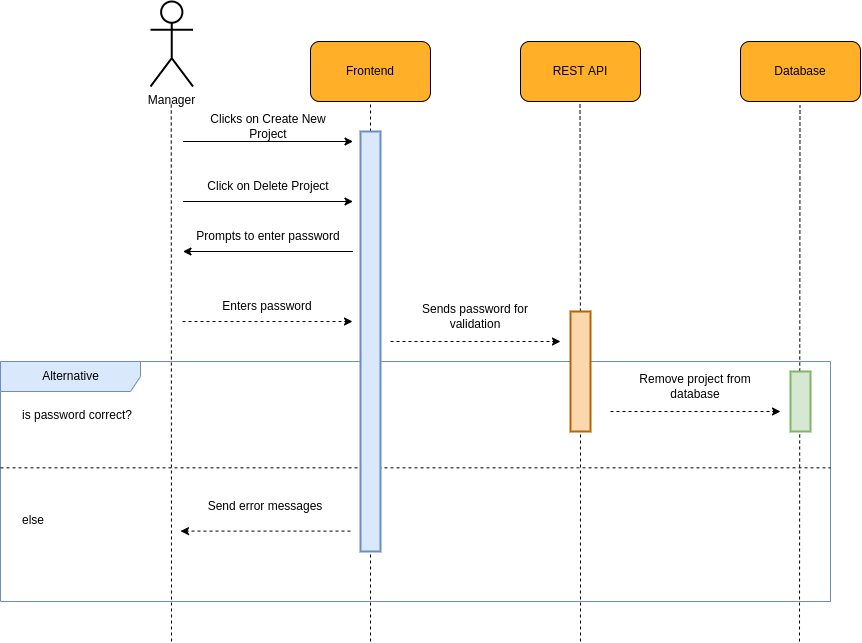
\includegraphics[scale=0.5]{./diagrams/sequence/seq-12.png}
    \caption{Sequence Diagram of UC-12}
    \label{fig:seq-12}
    
\end{figure}


\begin{figure}[H]
    \centering
    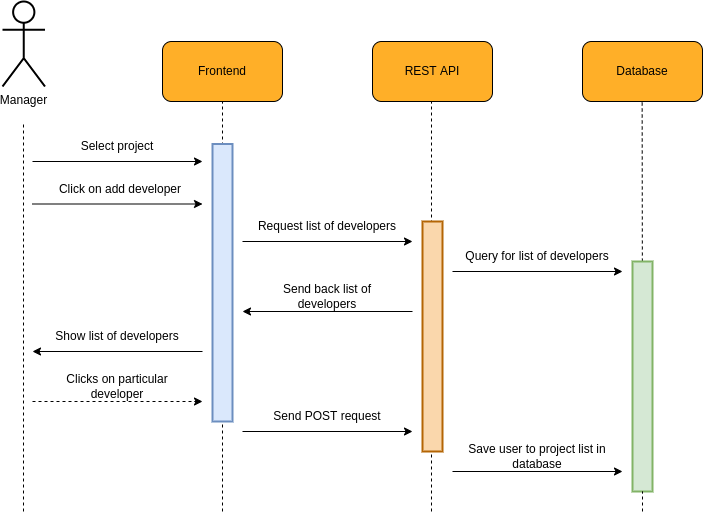
\includegraphics[scale=0.5]{./diagrams/sequence/seq-13.png}
    \caption{Sequence Diagram of UC-13}
    \label{fig:seq-13}
    
\end{figure}


\begin{figure}[H]
    \centering
    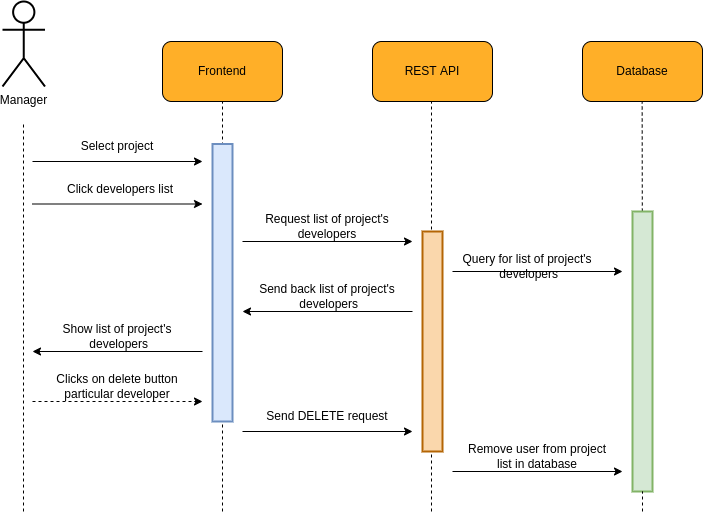
\includegraphics[scale=0.5]{./diagrams/sequence/seq-14.png}
    \caption{Sequence Diagram of UC-14}
    \label{fig:seq-14}
    
\end{figure}


\begin{figure}[H]
    \centering
    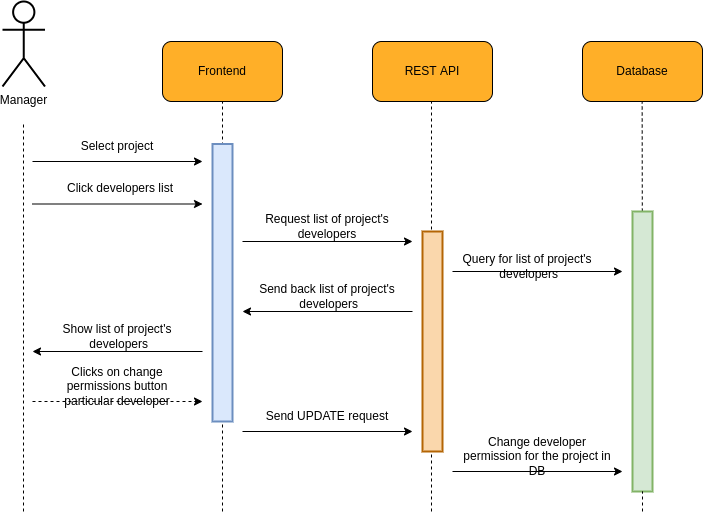
\includegraphics[scale=0.5]{./diagrams/sequence/seq-15.png}
    \caption{Sequence Diagram of UC-15}
    \label{fig:seq-15}
    
\end{figure}


\begin{figure}[H]
    \centering
    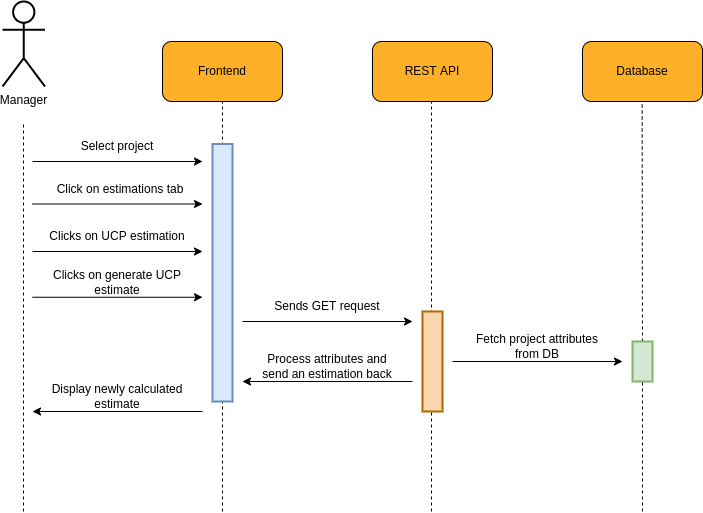
\includegraphics[scale=0.5]{./diagrams/sequence/seq-16.png}
    \caption{Sequence Diagram of UC-16}
    \label{fig:seq-16}
    
\end{figure}


\begin{figure}[H]
    \centering
    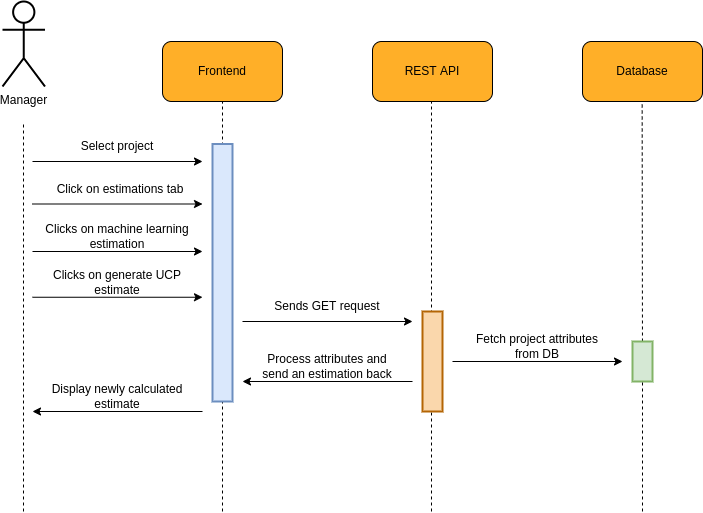
\includegraphics[scale=0.5]{./diagrams/sequence/seq-17.png}
    \caption{Sequence Diagram of UC-17}
    \label{fig:seq-17}
    
\end{figure}


\begin{figure}[H]
    \centering
    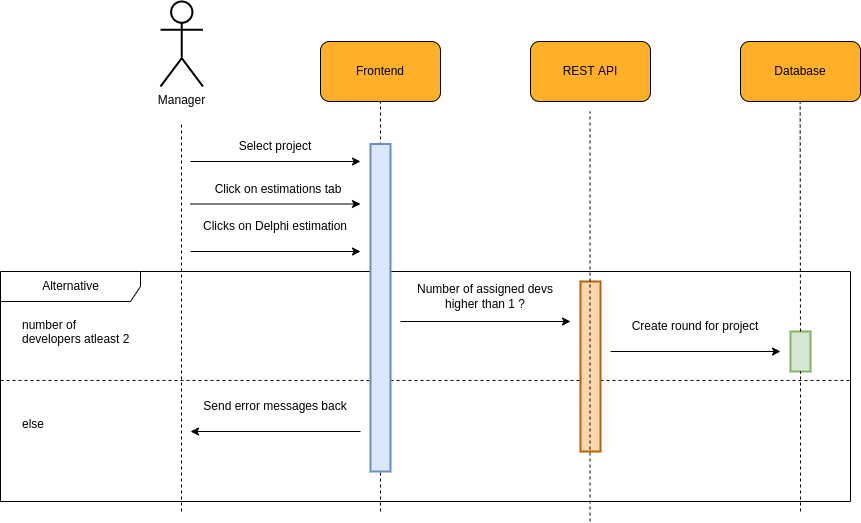
\includegraphics[scale=0.5]{./diagrams/sequence/seq-18.png}
    \caption{Sequence Diagram of UC-18}
    \label{fig:seq-18}
    
\end{figure}


\begin{figure}[H]
    \centering
    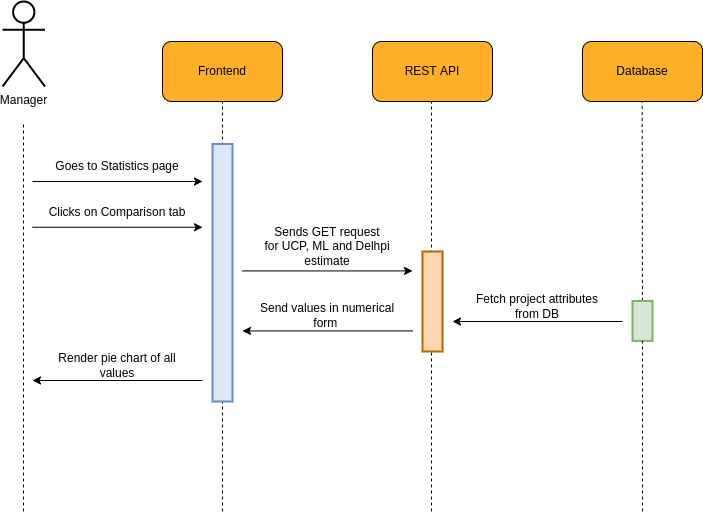
\includegraphics[scale=0.5]{./diagrams/sequence/seq-19.png}
    \caption{Sequence Diagram of UC-19}
    \label{fig:seq-19}
    
\end{figure}

